\documentclass[12pt,a4paper]{article}
\usepackage[utf8]{vietnam}
\usepackage{amsmath}
\usepackage{amsfonts}
\usepackage{amssymb}
\usepackage{graphicx}
\usepackage[left=2cm,right=2cm,top=2cm,bottom=2cm]{geometry}
% Gói lùi đầu dòng
\usepackage{indentfirst}
% Gói giúp mở ngoặc nhọn trái
\usepackage{cases}
% Gói giúp mở ngoặc nhọn phải
\usepackage{mathtools}
% Gói phục vụ cho hàm proof
\usepackage{amsthm}
% Gói dành cho header và footer
\usepackage{fancyhdr}
\pagestyle{fancy}
\fancyhf{} % Xoá header và footer mặc định
% Gói dùng cho khung
\usepackage{xcolor}
\usepackage{titlesec}
\usepackage{mdframed}
\newmdenv[linecolor=blue,skipabove=\topsep,skipbelow=\topsep,
leftmargin=1pt,rightmargin=0pt,
innerleftmargin=0pt,innerrightmargin=0pt]{mybox}
% Cài đặt header và footer
\lhead{Viện Toán ứng dụng và Tin học}
\rfoot{Trang \thepage}
% Gói để vẽ
\usepackage{tikz}
\begin{document}
	\thispagestyle{empty} % Định dạng header và footer cho từng đoạn
    \begin{mybox}
        \begin{center}
        		\fontsize{16}{24}\selectfont
        		\textbf{TRƯỜNG ĐẠI HỌC BÁCH KHOA HÀ NỘI 
        		\break
        		VIỆN TOÁN ỨNG DỤNG VÀ TIN HỌC}
        		\break
        		\break
        		\break
        		\break
        		\includegraphics[scale=0.15]{BK}
        		\break
        		        		
        		        		
        		\fontsize{24}{24}\selectfont
        		\textbf{SUY LUẬN THỐNG KÊ}
        		\break
         	\fontsize{16}{24}\selectfont        		        		
        		\textbf{BÀI TẬP VẼ HÌNH}
        		\break
        		\break
        		\break
        		
        		
        		
        		\textbf{
        		\fontsize{12}{18}\selectfont  
        			\begin{tabular}{ll}
        			Giảng viên: & PGS.TS. Nguyễn Thị Thuy Thuỷ \\ 
        			Sinh viên thực hiện: & Đoàn Minh Bảo \\ 
        			Lớp:  & Hệ thống thông tin quản lý (MI2) - K64 \\ 
        			\end{tabular} 
        		}
        		\break
        		\break
        		\break
        		\break
        		\break
        		\break
        		\fontsize{16}{24}\selectfont  
        		\textbf{HÀ NỘI - 2022}
        		\break
        		\break
        		\break
            		
		\end{center}         
    \end{mybox}
    
    \newpage
    
    	\tableofcontents 
    	
    	\newpage

    \section{Phân phối rời rạc}
		\subsection{Phân phối đều}
		$$
		P_X(x)=
		\begin{cases}
   			0.1 &  x = 0,1,...,9.  \\
			0 & \text{nếu trái lại.}
		\end{cases}
		$$
		\break		
		\textbf{Hình 1}
		
		
		
		\begin{tikzpicture}[domain=0:11]
			% Vẽ trục
			\draw [->] (-1,0) --(11,0) node [below] {$x$};
			\foreach \x in {1,2,3,4,5,6,7,8,9,10}
			\draw (\x,0.1)--(\x,-0.1) node [below] {\x};
			\draw[->] (0,-2) -- (0,4) node[above] {$f(x)$};
			\draw (-0.1,1) -- (0.1,1) node [left] {0.1};
			\draw (-0.4,-0.4) node {$O$};
			% Vẽ đồ thị
			\foreach \x in {0,1,2,3,4,5,6,7,8,9,10}
			\draw (\x,1)node [blue] {$\bullet$};
   			% domain là miền giá trị của x
   			% plot là đồ thị
		\end{tikzpicture}				
		\subsection{Phân phối Bernoulli}
		$$
		P_X(x)=
		\begin{cases}
   			1-p &  x = 0  \\
   			p & x=1 \\
			0 & \text{nếu trái lại.}
		\end{cases}
		$$
		\newpage
		\subsection{Phân phối nhị thức}
		$$
		P_X(x)=
		\begin{cases}
   			C_n^xp^x(1-p)^{n-x} &  x = 0  \\
			0 & \text{nếu trái lại.}
		\end{cases}
		$$
		\break
		\noindent\textbf{Hình 2}
		
		\begin{center}
		$n=20;p=0.5$		
		\end{center}
		
		
		\begin{tikzpicture}[domain=-0:21]
			% Vẽ trục
			\draw [->] (-0.5,0) --(17,0) node [below] {$x$};
			\foreach \x in {2,4,6,8,10,12,14,16,18,20}
			\draw (\x/1.5,0.1)--(\x/1.5,-0.1) node [below] {\x};
			\draw[->] (0,-2) -- (0,5) node[above] {$f(x)$};
			\foreach \y in {0.25}
			\draw (0.1,\y*15)--(-0.1,\y*15) node [left] {\y};
			\draw (-0.4,-0.4) node {$O$};
			% Vẽ đô thị
			\foreach \y[count =\i from 0] in 									{0.000001,0.000019,0.000181,0.001087,0.004621,0.014786,0.036964,0.073929,0.120134,0.160179,0.176197,0.160179,0.120134,0.073929,0.036964,0.014786,0.004621,0.001087,0.000181,0.000019,0.000001}
			\draw [blue](\i/1.5,\y*15) node{$\bullet$};
		\end{tikzpicture}
    
		\noindent\textbf{Hình 3}
		
		\begin{center}
		$n = 4; p =0.1$
		\end{center}
		
		
		\begin{tikzpicture}[domain=0:10]
			% Vẽ trục
			\draw [->] (-1,0) --(11,0) node [below] {$x$};
			\foreach \x in {1,2,3,4}
			\draw (\x*2,0.1)--(\x*2,-0.1) node [below] {\x};
			\draw[->] (0,-2) -- (0,7) node[above] {$f(x)$};
			\foreach \y in {0.1,0.2,0.3,0.6}
			\draw (0.1,\y*10)--(-0.1,\y*10) node [left] {\y};
			\draw (-0.4,-0.4) node {$O$};
			% Vẽ đồ thị
			\foreach \y[count =\i from 0] in {0.656100,0.291600,0.048600,0.003600,0.000100}
			\draw [blue](\i*2,\y*10) node{$\bullet$};
		\end{tikzpicture}
		\newpage
		\subsection{Phân phối Poisson}
		$$
		P_X(x)=
		\begin{cases}
   			\frac{e^{-\lambda}\lambda^x}{x!} $,$ k=0,1,2,...   x = 0,1,2...  \\
			0 & \text{nếu trái lại.}
		\end{cases}
		$$
	
	
		\noindent\textbf{Hình 4}
		
		\begin{center}
			$\lambda = 0.1; 3;7;10$
		\end{center}
	
		
		\begin{tikzpicture}[domain=0:10]
			% Vẽ trục			
			\draw [->] (-1,0) --(12,0) node [below] {$x$};
			\foreach \x in {1,2,3,4,5,6,7,8,9,10}
			\draw (\x,0.1)--(\x,-0.1) node [below] {\x};
			\draw[->] (0,-2) -- (0,6) node[above] {$f(x)$};
			\foreach \y in {0.2,0.4,0.6,0.8,1}
			\draw (0.1,\y*5)--(-0.1,\y*5) node [left] {\y};
			\draw (-0.4,-0.4) node {$O$};
			% Vẽ đồ thị
			\foreach \y[count =\i from 0] in {0.904837,0.090484,0.004524,0.000151,0.000004,0.000000,0.000000,0.000000,0.000000,0.000000,0.000000}
			\draw [blue](\i,\y*5) node{$\bullet$};
			
			\foreach \y[count =\i from 0] in {0.049787,0.149362,0.224042,0.224042,0.168032,0.100819,0.050410,0.021604,0.008102,0.002701,0.000810}
			\draw [red](\i,\y*5) node{$\bullet$};
			
			\foreach \y[count =\i from 0] in {0.000912,0.006383,0.022341,0.052129,0.091227,0.127717,0.149003,0.149003,0.130378,0.101405,0.070984}
			\draw [orange](\i,\y*5) node{$\bullet$};
			
			\foreach \y[count =\i from 0] in {0.000045,0.000454,0.002270,0.007567,0.018917,0.037834,0.063056,0.090080,0.112600,0.125111,0.125111}
			\draw [green](\i,\y*5) node{$\bullet$};
			
			\draw (10,5) node [blue] {$\bullet \lambda = 0.1$};
			\draw (10,4) node [red] {$\bullet \lambda = 3$};
			\draw (10,3) node [orange] {$\bullet \lambda = 7$};
			\draw (10,2) node [green] {$\bullet \lambda = 10$};
		\end{tikzpicture}
		
			
		\noindent \textbf{Hình 5 và 6}
		
		\begin{center}
			$\lambda = 5$
		\end{center}
		
		\begin{tikzpicture}[domain=0:10]
			% Vẽ trục
			\draw [->] (-1,0) --(12,0) node [below] {$x$};
			\foreach \x in {1,2,3,4,5,6,7,8,9,10}
			\draw (\x,0.1)--(\x,-0.1) node [below] {\x};
			\draw[->] (0,-2) -- (0,6) node[above] {$f(x)$};
			\foreach \y in {0.2,0.4}
			\draw (0.1,\y*10)--(-0.1,\y*10) node [left] {\y};
			\draw (-0.4,-0.4) node {$O$};
			% Vẽ đồ thị	
			\foreach \y[count =\i from 0] in {0.006738,0.033690,0.084225,0.140374,0.175468,0.175468,0.146223,0.104445,0.065278,0.036266,0.018133}
			\draw [blue](\i,\y*10) node{$\bullet$};
		\end{tikzpicture}
					
	\newpage
	\section{Phân phối liên tục} 
		\subsection{Phân phối đều}
			\subsubsection{Hàm mật độ}
		$$
		f_X(x)=
		\begin{cases}
   			\frac{1}{b-a} & \in [a;b] \\
   			0 & \notin [a;b]
		\end{cases}
		$$
		\noindent\textbf{Hình 7}
		
		\begin{tikzpicture}[domain=0:10]
			% Vẽ trục toạ độ
			\draw[->] (0,-2) -- (0,4) node[above] {$f(x)$};
			\draw [->] (-1,0) --(11,0) node [below] {$x$};
			\draw (2, -0.1) -- (2, 0.1) node [below] {$a$};
			\draw (5, -0.1) -- (5, 0.1) node [below] {$b$};
			\draw (-0.1,2) -- (0.1,2) node [left] {$\frac{1}{b-a}$};
			\draw (-0.4,-0.4) node {$O$};
			% Vẽ đồ thị
			\draw [blue] (2,2) -- (5,2);
			\draw [blue] (0,0) -- (2,0);
			\draw [blue] (5,0) -- (10,0);
		\end{tikzpicture}			
		
		

			\subsubsection{Hàm phân phối}	
		$$
		F_X(x)=
		\begin{cases}
   			0 & x <= a \\
   			\frac{x-a}{b-a} & a<x<=b \\
   			1 & x>b
		\end{cases}
		$$
			\noindent\textbf{Hình 8}
			
		\begin{tikzpicture}[domain=0:10]
			% Vẽ trục toạ độ
			\draw[->] (0,-2) -- (0,4) node[above] {$f(x)$};
			\draw [->] (-1,0) --(11,0) node [below] {$x$};
			\draw (2, -0.1) -- (2, 0.1) node [below] {$a$};
			\draw (5, -0.1) -- (5, 0.1) node [below] {$b$};
			\draw (-0.1,2) -- (0.1,2) node [left] {1};
			\draw (-0.4,-0.4) node {$O$};
			% Vẽ đồ thị
			\draw [thick,blue] (0,0) -- (2,0) -- (5,2) -- (9,2);	
		\end{tikzpicture}	
		\subsection{Phân phối mũ}
			\subsubsection{Hàm mật độ}
		$$
		f_X(x)=
		\begin{cases}
   			\lambda e^{-\lambda x} & x >= 0 \\
   			0 & x < 0 
		\end{cases}
		$$
		
		
		\noindent\textbf{Hình 9}
		
		\begin{center}
			$\lambda = 0.1; 0.5; 3$
		\end{center}
		
		\begin{tikzpicture}[domain=0:11]
			% Vẽ trục
			\draw [->] (-1,0) --(11,0) node [below] {$x$};
			\foreach \x in {1,2,3,4,5,6,7,8,9,10}
			\draw (\x,0.1)--(\x,-0.1) node [below] {\x};
			\draw[->] (0,-2) -- (0,6) node[above] {$f(x)$};
			\foreach \y in {0.2,0.4,0.6,0.8,1}
			\draw (0.1,\y*5)--(-0.1,\y*5) node [left] {\y};
			\draw (-0.4,-0.4) node {$O$};
			% Vẽ đồ thị
			\draw [blue] plot(\x,{5*0.1*e^(-0.1*\x)});
			\draw [red] plot(\x,{5*0.5*e^(-0.5*\x)});
			\draw [green, domain=0.3:10] plot(\x,{5*3*e^(-3*\x)});
			\draw (10,5) node [blue] {$\bullet \lambda = 0.1$};
			\draw (10,4) node [red] {$\bullet \lambda = 0.5$};
			\draw (10,3) node [green] {$\bullet \lambda = 3$};	
		\end{tikzpicture}
			
			\subsubsection{Hàm phân phối}
		$$
		F_X(x)=
		\begin{cases}
   			1 - e^{-\lambda x} & x >= 0 \\
   			0 & x < 0 
		\end{cases}
		$$
		\newpage
		\subsection{Phân phối chuẩn}
			\subsubsection{Phân phối chuẩn}
		\begin{center}
			$f_X(x) = \frac{1}{\sigma\sqrt{2\pi}}e^{-\frac{\left(x-\mu\right)^2}{2\sigma^2}} $			
		\end{center}
					
		\noindent \textbf{Hình 10}
		
		\begin{center}
			$\mu=1;\sigma=0.25$
		\end{center}
		\begin{tikzpicture}[domain=-1:3.5]
			% Vẽ trục
			\draw [->] (-3,0) --(7,0) node [below] {$x$};
			\foreach \x in {0.5,1,1.5,2,2.5,3}
			\draw (\x*2,0.1)--(\x*2,-0.1) node [below] {\x};
			\draw[->] (0,-2) -- (0,6) node[above] {$f(x)$};
			\foreach \y in {0.5,1,1.5,2}
			\draw (0.1,\y*2)--(-0.1,\y*2) node [left] {\y};
			\draw (-0.4,-0.4) node {$O$};
			%Vẽ đồ thị
			\draw [blue,samples = 200] plot(2*\x, {2*e^((-(\x-1)^2)/2/0.25^2)/0.25/2.506628 });	
		\end{tikzpicture}
					
					
		\noindent \textbf{Hình 11}
		
		\begin{center}
			$\mu_1=1 < \mu_2=2$			
			$\sigma_1 = \sigma_2=0.25$
		\end{center}
		
		\begin{tikzpicture}[domain=-1:3.5]
			% Vẽ trục
			\draw [->] (-3,0) --(7,0) node [below] {$x$};			
			\draw[->] (0,-2) -- (0,6) node[above] {$f(x)$};
			\foreach \x in {0.5,1,1.5,2,2.5,3}
			\draw (\x*2,0.1)--(\x*2,-0.1) node [below] {\x};
			\draw[->] (0,-2) -- (0,6) node[above] {$f(x)$};
			\foreach \y in {0.5,1,1.5,2}
			\draw (0.1,\y*2)--(-0.1,\y*2) node [left] {\y};
			\draw (-0.4,-0.4) node {$O$};
			% Vẽ đồ thị
			\draw [blue,samples = 200] plot(2*\x, {2*e^((-(\x-1)^2)/2/0.25^2)/0.25/2.506628 });
			\draw [red,samples = 200] plot(2*\x, {2*e^((-(\x-2)^2)/2/0.25^2)/0.25/2.506628 });
			
			\draw (7,6) node [blue] {$\bullet$ Đường 1};
			\draw (7,5) node [red] {$\bullet $ Đường 2};	
		\end{tikzpicture}
			
		\newpage
		\noindent\textbf{Hình 12}
		
		\begin{center}
			$\mu_1=1 = \mu_2=1$		
				
			$\sigma_1 = 0.25 < \sigma_2=0.35$
		\end{center}
		
		\begin{tikzpicture}[domain=-1:3.5 ]
			% Vẽ trục
			\draw [->] (-3,0) --(7,0) node [below] {$x$};		
			\draw[->] (0,-2) -- (0,6) node[above] {$f(x)$};
			\foreach \x in {0.5,1,1.5,2,2.5,3}
			\draw (\x*2,0.1)--(\x*2,-0.1) node [below] {\x};
			\draw[->] (0,-2) -- (0,6) node[above] {$f(x)$};
			\foreach \y in {0.5,1,1.5,2}
			\draw (0.1,\y*2)--(-0.1,\y*2) node [left] {\y};
			\draw (-0.4,-0.4) node {$O$};
			% Vẽ đồ thị
			\draw [blue,samples = 200] plot(2*\x, {2*e^((-(\x-1)^2)/2/0.25^2)/0.25/2.506628 });
			\draw [red,samples = 200] plot(2*\x, {2*e^((-(\x-1)^2)/2/0.35^2)/0.35/2.506628 });
			
			\draw (7,6) node [blue] {$\bullet$ Đường 1};
			\draw (7,5) node [red] {$\bullet $ Đường 2};	
			\end{tikzpicture}
			
			
		\noindent \textbf{Hình 13}
		
		\begin{center}
			$\mu_1=1 <\mu_2=2$
			
			$\sigma_1 = 0.25 < \sigma_2=0.35$
		\end{center}
		
		\begin{tikzpicture}[domain=-1:3.5 ]
			% Vẽ trục
			\draw [->] (-3,0) --(9,0) node [below] {$x$};	
			\draw[->] (0,-2) -- (0,6) node[above] {$f(x)$};
			\foreach \x in {0.5,1,1.5,2,2.5,3,3.5}
			\draw (\x*2,0.1)--(\x*2,-0.1) node [below] {\x};
			\draw[->] (0,-2) -- (0,6) node[above] {$f(x)$};
			\foreach \y in {0.5,1,1.5,2}
			\draw (0.1,\y*2)--(-0.1,\y*2) node [left] {\y};
			\draw (-0.4,-0.4) node {$O$};
			% Vẽ đồ thị
			\draw [blue,samples = 200] plot(2*\x, {2*e^((-(\x-1)^2)/2/0.25^2)/0.25/2.506628 });
			\draw [red,samples = 200] plot(2*\x, {2*e^((-(\x-2)^2)/2/0.35^2)/0.35/2.506628 });
			
			\draw (7,6) node [blue] {$\bullet$ Đường 1};
			\draw (7,5) node [red] {$\bullet $ Đường 2};	
		\end{tikzpicture}
		\newpage
			\subsubsection{Phân phối chuẩn tắc}			
		\begin{center}			
			$\varphi(z) = \frac{1}{\sqrt{2\pi}}e^{-\frac{z^2}{2}} $		
		\end{center}
					
		\noindent \textbf{Hình 14}
		
		
		\begin{center}
			$\mu=0;\sigma=1$
		\end{center}
		\begin{tikzpicture}[domain=-3.5:3.5]
			% Vẽ trục
			\draw [->] (-7,0) --(7,0) node [below] {$z$};
			\foreach \x in {-3,-2.5,-2,-1.5,-1,-0.5,0.5,1,1.5,2,2.5,3}
			\draw (\x*2,0.1)--(\x*2,-0.1) node [below] {\x};
			\draw[->] (0,-2) -- (0,4) node[above] {$\varphi(z)$};
			\foreach \y in {0.5}
			\draw (0.1,\y*6)--(-0.1,\y*6) node [left] {\y};
			\draw (-0.4,-0.4) node {$O$};
			% Vẽ đồ thị
			\draw [blue,samples = 200] plot(2*\x, {6*e^((-(\x)^2)/2)/2.506628 });
		\end{tikzpicture}
					
		\begin{center}
			$\Phi(z) = \frac{1}{\sqrt{2\pi}}\displaystyle\int_{-\infty}^z(e^{\frac{-t^2}{2}})dt $		
		\end{center}		
			
		\noindent \textbf{Hình 15}
		
		
		\begin{center}
			$\mu=0;\sigma=1; z=2$
		\end{center}
		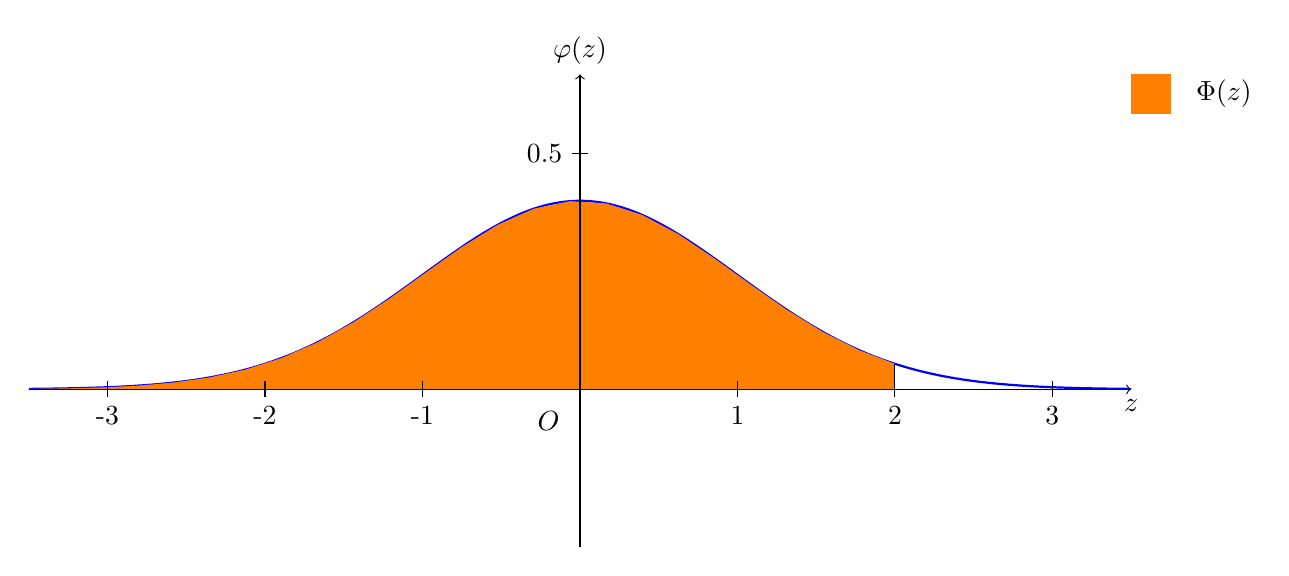
\begin{tikzpicture}[domain=-3.5:3.5]		
			% Vẽ đồ thị		
			\draw [blue,thick,samples = 200] plot(2*\x, {6*e^((-(\x)^2)/2/1^2)/2.506628 });	
			\fill [orange, domain=-3.5:2, variable=\x]
(-7,0)--plot(2*\x,{6*e^((-(\x)^2)/2/1^2)/2.506628 })--(4,0);
			\draw (2*2, 0.323945) -- (4,0);			
			\fill [orange] (7.5,3.5) --(7,3.5) --(7,4) -- (7.5,4); 
			\draw (7.7,3.75) node [right,black] {$\Phi(z)$};
			% Vẽ trục
			\draw [->] (-7,0) --(7,0) node [below] {$z$};
			\draw[->] (0,-2) -- (0,4) node[above] {$\varphi(z)$};
 			\foreach \x in {-3,-2,-1,1,2,3}
			\draw (\x*2,0.1)--(\x*2,-0.1) node [below] {\x};
			\foreach \x in {0.5}
			\draw (0.1,\x*6)--(-0.1,\x*6) node [left] {\x};
			\draw (-0.4,-0.4) node {$O$};
		\end{tikzpicture}
			
		\newpage
  		\noindent \textbf{Hình 16}
		
		\begin{center}
			$\mu=0;\sigma=1; z=1$
		\end{center}
		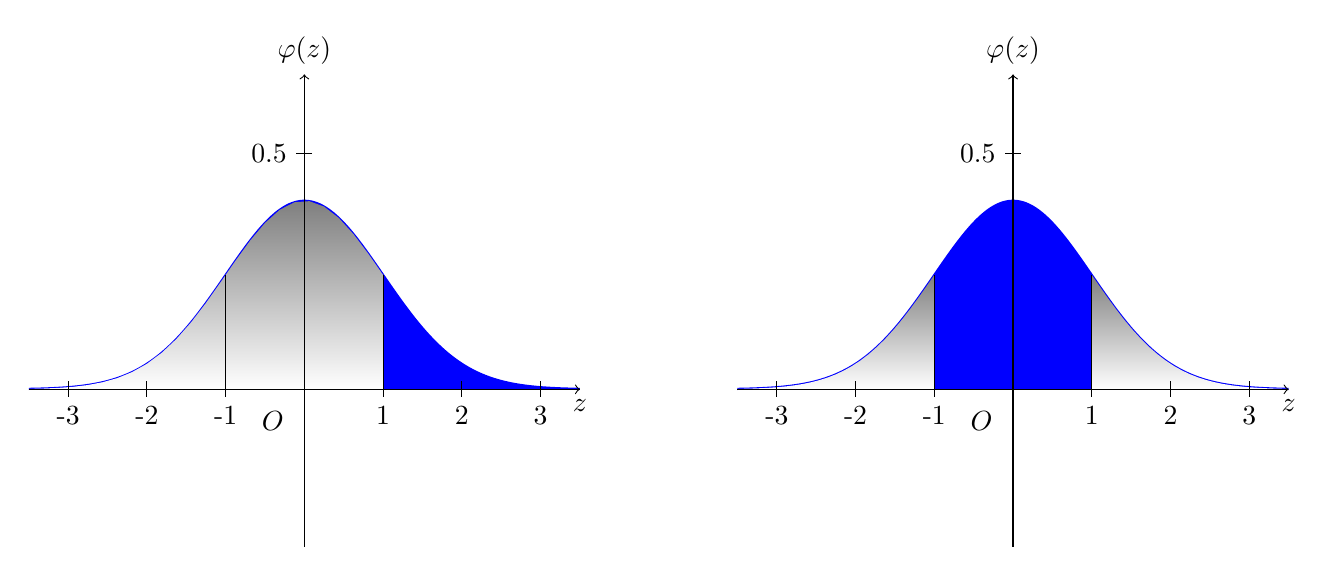
\begin{tikzpicture}[domain=-3.5:3.5]
			% Đồ thị 1
			% Vẽ đồ thị		
			\draw [blue,thick,samples = 200] plot(\x, {6*e^((-(\x)^2)/2/1^2)/2.506628});
			\shade [blue, domain=-3.5:1, variable=\x]
(-3.5, 0) --  plot(\x, {6*e^((-(\x)^2)/2/1^2)/2.506628 }) -- (1, 0);
			\fill [blue,domain=1:3.5, variable=\x]
(1, 0) --  plot(\x, {6*e^((-(\x)^2)/2/1^2)/2.506628 })-- (3.5, 0); 	
			\draw (1, 1.451824) -- (1, 0);
			\draw (-1, 1.451824) -- (-1, 0);
			% Vẽ trục
			\draw [->] (-3.5,0) --(3.5,0) node [below] {$z$};
			\draw[->] (0,-2) -- (0,4) node[above] {$\varphi(z)$};
 			\foreach \x in {-3,-2,-1,1,2,3}
			\draw (\x,0.1)--(\x,-0.1) node [below] {\x};
			\foreach \x in {0.5}
			\draw (0.1,\x*6)--(-0.1,\x*6) node [left] {\x};
			\draw (-0.4,-0.4) node {$O$};
			% Đồ thị 2 (+9 cho các thông số của x)
			% Vẽ đồ thị		
			\draw [blue,thick,samples = 200] plot(\x+9, {6*e^((-(\x)^2)/2/1^2)/2.506628});
			\fill [blue, domain=-3.5:1, variable=\x]
(-3.5+9, 0) --  plot(\x+9, {6*e^((-(\x)^2)/2/1^2)/2.506628 }) -- (1+9, 0);
			\shade [blue,domain=1:3.5, variable=\x]
(1+9,0) --  plot(\x+9, {6*e^((-(\x)^2)/2/1^2)/2.506628 })-- (3.5+9, 0); 			\shade [blue,domain=-3.5:-1, variable=\x]
(-3.5+9,0) --  plot(\x+9, {6*e^((-(\x)^2)/2/1^2)/2.506628 })-- (-1+9, 0);
			\draw (1+9, 1.451824) -- (1+9, 0);
			\draw (-1+9, 1.451824) -- (-1+9, 0);
			% Vẽ trục
			\draw [->] (-3.5+9,0) --(3.5+9,0) node [below] {$z$};
			\draw[->] (0+9,-2) -- (0+9,4) node[above] {$\varphi(z)$};
 			\foreach \x in {-3,-2,-1,1,2,3}
			\draw (\x+9,0.1)--(\x+9,-0.1) node [below] {\x};
			\foreach \x in {0.5}
			\draw (0.1+9,\x*6)--(-0.1+9,\x*6) node [left] {\x};
			\draw (-0.4+9,-0.4) node {$O$};
		\end{tikzpicture}
			
			\subsubsection{Xác suất để biến ngẫu nhiên có phân phối chuẩn nhận giá trị trong khoảng}
			
    		\noindent \textbf{Hình 17}
    		
		
		\begin{center}
			$ P(\mu-\sigma < X < \mu+\sigma) = 0.6827 $	
					
			$ P(\mu-2\sigma < X < \mu+2\sigma) = 0.9545 $		
				
			$ P(\mu-3\sigma < X < \mu+3\sigma) = 0.9973 $
		\end{center}
		
		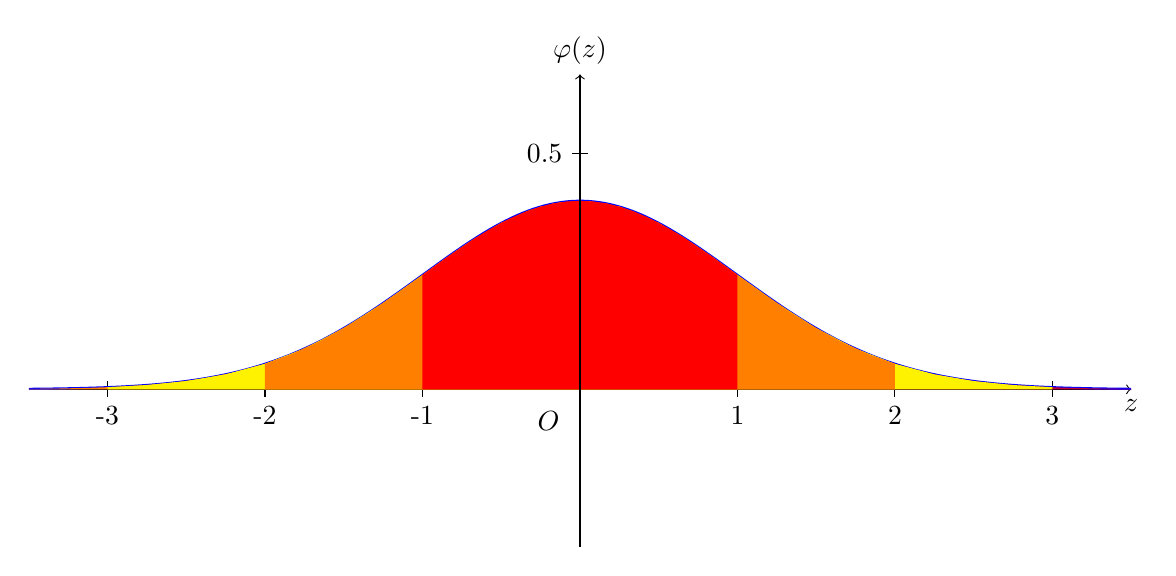
\begin{tikzpicture}[domain=-3.5:3.5]
			% Vẽ trục
			\draw [->] (-7,0) --(7,0) node [below] {$z$};
			 \foreach \x in {-3,-2,-1,1,2,3}
			\draw (\x*2,0.1)--(\x*2,-0.1) node [below] {\x};
			\foreach \x in {0.5}
			\draw (0.1,\x*6)--(-0.1,\x*6) node [left] {\x};
			\draw (-0.4,-0.4) node {$O$};
			% Vẽ đô thị		
			\draw [blue,thick,samples = 200] plot(2*\x, {6*e^((-(\x)^2)/2/1^2)/2.506628 });
			\fill [orange, domain=-3.5:1, variable=\x]
(-7, 0) -- plot(2*\x,{6*e^((-(\x)^2)/2/1^2)/2.506628 }) -- (2, 0);
 			\fill [purple, domain=1:3.5, variable=\x]
(2, 0) --  plot(2*\x,{6*e^((-(\x)^2)/2/1^2)/2.506628 }) -- (7, 0);
			\draw (1*2, 1.451824) -- (2, 0);					
			\fill [ yellow, domain=-3:3, variable=\x]
(-6, 0) --  plot(2*\x, {6*e^((-(\x)^2)/2/1^2)/2.506628 }) -- (6, 0);
  			\fill [ orange, domain=-2:2, variable=\x]
(-4, 0)--  plot(2*\x,{6*e^((-(\x)^2)/2/1^2)/2.506628 })-- (4, 0);
  			\fill [ red, domain=-1:1, variable=\x]
(-2, 0) --  plot(2*\x, {6*e^((-(\x)^2)/2/1^2)/2.506628 }) -- (2, 0);		
			 \draw[->] (0,-2) -- (0,4) node[above] {$\varphi(z)$};
		\end{tikzpicture}
					
		\newpage
		\noindent \textbf{Hình 18}
		
		
		\begin{center}
			$n=15;p=0.4$			
				
			$\mu=6;\sigma^2=3.6$
		\end{center}
		\begin{tikzpicture}[domain=-0:12.5]
			% Vẽ trục
			\draw [->] (-0.5,0) --(17,0) node [below] {$z$};
			\foreach \x in {2,4,6,8,10,12,14,16}
			\draw (\x,0.1)--(\x,-0.1) node [below] {\x};
			\draw[->] (0,-2) -- (0,5) node[above] {$\varphi(z)$};
			\foreach \y in {0.25}
			\draw (0.1,\y*15)--(-0.1,\y*15) node [left] {\y};
			\draw (-0.4,-0.4) node {$O$};
			% Vẽ đồ thị
			\draw [red,samples = 200] plot(\x, {15*e^((-(\x-6)^2)/2/3.6)/2.506628/1.8973 });	
			\foreach \y[count =\i from 0] in {0.000470,0.004702,0.021942,0.063388,0.126776,0.185938,0.206598,0.177084,0.118056,0.061214,0.024486,0.007420,0.001649,0.000254,0.000024,0.000001}
			\draw [blue] (-0.5+1*\i,0) rectangle ++(1,15*\y);
		\end{tikzpicture}
									
		\noindent \textbf{Hình 19}


		\begin{center}
			$n=25;p=0.5$		
			
			$\mu=12.5;\sigma=2.5$
		\end{center}
		\begin{tikzpicture}[domain=-0:25]
			% Vẽ trục
			\draw [->] (-0.5,0) --(17,0) node [below] {$z$};
			\foreach \x in {2,4,6,8,10,12,14,16,18,20,22,24}
			\draw (\x/1.5,0.1)--(\x/1.5,-0.1) node [below] {\x};
			\draw[->] (0,-2) -- (0,5) node[above] {$\varphi(z)$};
			\foreach \y in {0.25}
			\draw (0.1,\y*15)--(-0.1,\y*15) node [left] {\y};
			\draw (-0.4,-0.4) node {$O$};
			% Vẽ đồ thị		
			\draw [red,samples = 200] plot(\x/1.5, {15*e^((-(\x-12.5)^2)/2/6.25)/2.506628/2.5 });				
			\foreach \y[count =\i from 0] in 
{0.000000,0.000001,0.000009,0.000069,0.000377,0.001583,0.005278,0.014326,0.032233,0.060885,0.097417
,0.132841,0.154981,0.154981,0.132841,0.097417,0.060885,0.032233,0.014326,0.005278,0.001583,0.000377,0.000069,0.000009,0.000001,0.000000}			
			\draw [blue] (-0.5/1.5+1*\i/1.5,0) rectangle + +(1/1.5,15*\y);
		\end{tikzpicture}
					
					
		\newpage		
		\noindent \textbf{Hình 20}
		
		
		\begin{center}
			$n=25;p=0.1$			
			
			$\mu=2.5;\sigma=1.5$
		\end{center}
		\begin{tikzpicture}[domain=-0:25]
			% Vẽ trục
			\draw [->] (-0.5,0) --(17,0) node [below] {$z$};
			\foreach \x in {2,4,6,8,10,12,14,16,18,20,22,24}
			\draw (\x/1.5,0.1)--(\x/1.5,-0.1) node [below] {\x};
			\draw[->] (0,-2) -- (0,5) node[above] {$\varphi(z)$};
			\foreach \y in {0.25}
			\draw (0.1,\y*15)--(-0.1,\y*15) node [left] {\y};
			\draw (-0.4,-0.4) node {$O$};
			% Vẽ đồ thị			
			\draw [red,samples = 200] plot(\x/1.5, {15*e^((-(\x-2.5)^2)/2/2.25)/2.506628/1.5 });			
			\foreach \y[count =\i from 0] in {0.071790,0.199416,0.265888,0.226497,0.138415,0.064594,0.023924,0.007215,0.001804,0.000379,0.000067,0.000010,0.000001,0.000000,0.000000,0.000000,0.000000,0.000000,0.000000,0.000000,0.000000,0.000000,0.000000,0.000000,0.000000,0.000000}
			\draw [blue] (-0.5/1.5+1*\i/1.5,0) rectangle ++(1/1.5,15*\y);
		\end{tikzpicture}
    
\end{document}


























